\documentclass[11pt, oneside]{article} 
\usepackage{amsmath, amsthm, amssymb, wasysym, verbatim, bbm, color, geometry}
\usepackage{amsfonts}
\usepackage{csquotes}
% \usepackage{polski}
\usepackage[english]{babel}
\usepackage[nottoc]{tocbibind}
\usepackage{caption}
\usepackage{subcaption}
\usepackage{float}
\usepackage{graphicx}
\usepackage{circuitikz}
\usepackage{listings}
\usepackage{float}


\definecolor{codegreen}{rgb}{0,0.6,0}
\definecolor{codegray}{rgb}{0.5,0.5,0.5}
\definecolor{codepurple}{rgb}{0.58,0,0.82}
\definecolor{backcolour}{rgb}{0.95,0.95,0.92}

\lstdefinestyle{mystyle}{
    backgroundcolor=\color{backcolour},   
    commentstyle=\color{codegreen},
    keywordstyle=\color{magenta},
    numberstyle=\tiny\color{codegray},
    stringstyle=\color{codepurple},
    basicstyle=\ttfamily\footnotesize,
    breakatwhitespace=false,         
    breaklines=true,                 
    captionpos=b,                    
    keepspaces=true,                 
    numbers=left,                    
    numbersep=5pt,                  
    showspaces=false,                
    showstringspaces=false,
    showtabs=false,                  
    tabsize=2
}
\lstset{style=mystyle}

% \ctikzset{current arrow scale=1.5} 
\usepackage{hyperref} % Loads the hyperref package for hyperlinks
\usepackage{enumitem}
\usepackage{tikz}
\usepackage{pgfplots}
\usepackage[T1]{fontenc}
\usepackage{algorithm}
\usepackage{algpseudocode}
\usepackage{amsfonts}
\usepackage{mathbbol}

\catcode`_=\active
\def_#1{\sb{\mathrm{#1}}}


\pgfplotsset{compat=1.18} % Set the compatibility level for pg
\usetikzlibrary{shapes.geometric, arrows, positioning, fit, backgrounds}

\hypersetup{
    colorlinks=true,
    linkcolor=blue,
    citecolor=cyan,
    urlcolor=blue!60,
    breaklinks=true,
}





\newcommand{\workSource}[2]{Text available at: \href{#1}{#2}}



\DeclareMathSizes{12}{12}{10}{8}
\makeatletter
\renewcommand\normalsize{%
\@setfontsize\normalsize{12pt}{13.5pt}% Will look incredibly crabbed if line height is too small
\abovedisplayskip 10\p@ \@plus2\p@ \@minus5\p@%
\abovedisplayshortskip \z@ \@plus2\p@%
\belowdisplayshortskip 5\p@ \@plus2\p@ \@minus3\p@%
\belowdisplayskip \abovedisplayskip%
\let\@listi\@listI%
}
\normalsize  
\makeatother

\newcommand{\der}{{\rm d}}
\newcommand{\R}{\mathcal{R}}
\newcommand{\C}{\mathcal{C}}
\newcommand{\M}{\mathcal{M}}
\newcommand{\G}{\mathcal{G}}
\newcommand{\Ron}{R_{\rm ON}}
\newcommand{\Roff}{R_{\rm OFF}}
\newcommand{\von}{V_{\rm ON}}
\newcommand{\voff}{V_{\rm OFF}}
\newcommand{\q}{q}
\newcommand{\ua}{v}
\newcommand{\ia}{i}
\newcommand{\phia}{\varphi}
\newcommand{\xw}{x}
\newcommand{\dert}[1]{\frac{{\rm d} {#1}}{{\rm d} t} }
\newcommand{\inv}[1]{\frac{1}{#1} }
\newcommand{\equal}{=}


\usepackage[style=numeric, 
            backend=biber,
           ]{biblatex}
           
\addbibresource{bibliography.bib} % Replace with your .bib file name

\geometry{tmargin=.75in, bmargin=.75in, lmargin=.75in, rmargin = .75in}  

% \usepackage{fontspec}
% \setmainfont[]{Palatino}

\newcommand{\Cdot}{\boldsymbol{\cdot}}

\newtheorem{thm}{Theorem}
\newtheorem{defn}{Definition}
\newtheorem{conv}{Convention}
\newtheorem{rem}{Remark}
\newtheorem{lem}{Lemma}
\newtheorem{cor}{Corollary}


\title{Reservoir computing}
\author{Karol Bednarz}
% \date{Rok akademicki 2024--2025}
\date{\today}

\begin{document}

\maketitle
\tableofcontents

\vspace{.25in}

\newcommand{\Todo}[1]{\textcolor                {red}{\textbf{TODO:} #1}}


\section{State of the art in reservoir computing}

\subsection{ESN - Echo State Network}
\subsubsection{Principles of reservoir computing}
Based on the~\autocite{Bai2023}:
The state of reservoir dynamics can be expressed as:
\begin{equation}
    h_t = f \big((1-k) \cdot u_t \cdot W_{in} + k\cdot h_{\mathrm{t-1}} \cdot W_h + y_{\mathrm{t-1}} \cdot W_{1b} + b \big)
\end{equation}
Where:
\begin{itemize}[noitemsep, leftmargin=4cm, label={}]
    \item [\(h_{t-1}\)] -- are the reservoir state respectively, from the previous time step,
    \item [\(u_t\)] -- is the observed data at time step \(t\),
    \item [\(y_{t-1}\)] -- is the the predicted output state \(t-1\),
    \item [\(W_{in} \in \mathbb{R}^{N_u \times N_h}\)] -- is the input weight matrix,
    \item [\(W_h \in \mathbb{R}^{N_h \times N_h}\)] -- is the internal weight matrix,
    \item [\(W_{1b} \in \mathbb{R}^{N_h \times N_y}\)] -- is the output fedback weight matrix,
    \item [\(b \in \mathbb{R}^{N_h}\)] -- is the bias vector.
    \item [\(f\)] -- is the activation function, typically \(\tanh\) or \(\mathrm{sigmoid}\),
    \item [\(k\)] -- is the leaking rate, typically \(k \in [0.1, 0.3]\).
\end{itemize}


With the computed reservoir dynamics, the output can be then obtained by:
\begin{equation}
    y_t = h_t \cdot W_{\mathrm{out}}
\end{equation}
Where:
\begin{itemize}[noitemsep, leftmargin=4cm, label={}]
    \item [\(W_{\mathrm{out}} \in \mathbb{R}^{N_h \times N_y}\)] -- is the output weight matrix.
\end{itemize}

\subsubsection{Echo state property}

Any system that changes in a nonlinear way can work as the reservoir. However, starting a nonlinear system with random connection strengths creates problems.
The reservoir is a system that feeds its outputs back into itself. This can make it unstable if the connection strengths aren't set up correctly. For example, if the internal connections are too strong, the system might get stuck giving the same output regardless of what input it receives. The random connection strengths must be chosen so the system doesn't grow out of control.
For the system to work well, it must follow something called the "echo state property." This rule ensures that the reservoir's behavior eventually depends on the input signal rather than just its starting conditions.
To meet this requirement, the internal connection matrix \(W_h\) is first set up using random values between -1 and 1. This matrix is then adjusted one time according to the echo state property rule:

\begin{align}
    W'_h          & = \alpha \odot {W_h}                                             \\
    W_h^{\dagger} & = \frac{\rho  W_h}{\left\lvert \lambda_{max}(W_h) \right\rvert }
\end{align}
Where:
\begin{itemize}[noitemsep, leftmargin=4cm, label={}]
    \item [\(\rho \in (0,1)\)] -- is the spectral radius, typically \(\rho \in [0.9, 1]\)
    \item [\(\lambda_{max}(W_h)\)] -- is the largest eigenvalue of \(W_h \).
    \item[\(\alpha \in (0,1)\)] -- is the sparsity coefficient, typically \(\alpha \in [0.1, 0.3]\).
\end{itemize}
The spectral radius is a parameter that determines the amount of nonlinear interaction of input components through time.

Due to the recursive nature of the reservoir layer,
such dynamics reflect trajectories of the past historical input—the short-term memory (known as the fading memory). As another critical property for computing the RC principle, short-term memory can be
quantitative measured by the coefficient of memory
capacity


\begin{equation}
    MC = \sum_{k=1}^{\infty} MC_k =
    \sum_{k=1}^{\infty} d^2(u_{t-k}, y_t) =  \sum_{k=1}^{\infty} \frac{\mathrm{cov}^2(u_{t-k}, y_t)}{\sigma^2(u_t) \sigma^2(y_t)}
\end{equation}

Where:
\begin{itemize}[noitemsep, leftmargin=4cm, label={}]
    \item [\(d^2(u_{t-k}, y_t)\)] -- is the square of the correlation coefficient between the output \(y_t\) and the input \(u_{t-k }\) with a delay of \(k\) time steps,
\end{itemize}

According to the Lyapunov stability analysis, a large memory capacity is needed to compute the RC principle, which can be achieved at the asymptotically stable region.


\subsubsection{Learning algorithm}
The training of the reservoir computing model involves adjusting only the output weights \(W_{\mathrm{out}}\). The input weights \(W_{in}\), internal weights \(W_h\), and feedback weights \(W_{1b}\) are typically initialized randomly and remain fixed during training. The training process can be summarized in the following steps:

\begin{equation}
    Y = H \cdot W_{out}
\end{equation}
Where:
\begin{itemize}[noitemsep, leftmargin=4cm, label={}]
    \item [\(Y \in \mathbb{R}^{T \times N_y}\)] -- is the matrix of target outputs for all time steps,
    \item [\(H \in \mathbb{R}^{T \times N_h}\)] -- is the matrix of reservoir states for all time steps,
    \item [\(T\)] -- is the total number of time steps.
\end{itemize}

In general, the \(W_{out}\) can be directly obtained by calculating the Moore-Penrose pseudoinverse of the reservoir states matrix H with respect to the target outputs matrix Y:

\begin{equation}
    W_{out} = Y \cdot H^{T} \cdot (H \cdot H^{T} + \eta I)^{-1}
\end{equation}
Where:
\begin{itemize}[noitemsep, leftmargin=2cm, label={}]
    \item [\(H^{T}\)] -- is the transpose of matrix H,
    \item [\(\eta\)] -- is the regularization parameter, typically \(\eta \in [10^{-6}, 10^{-2}]\),
    \item [\(I\)] -- is the identity matrix of size \(N_h \times N_h\).
\end{itemize}


\subsubsection{Model development}


The echo state network (ESN)  and the liquid state machine (LSM)  are the two representations of RC.  While ESN and LSM are topographically equivalent, the former adopts the actual numerical data from the input to compute the network dynamics, and the latter adopts the spiking signal to represent the spatiotemporal pattern. \textbf{The LSM can be also seen as a SNN, where the reservoir has numerous leaky integrate-and-fire (LIF) neurons interconnected with the same recursive nature as in ESN}. As the spiking event is involved, the training of LSM generally relies on the spike-timing-dependent plasticity (STDP)  and short-term plasticity (STP), among other training methods for spiking networks.


\subsection{Time-delayed reservoir computing}
Based on~\autocite{Grigoryeva2016, Parlitz2024, Ortn2015}.

The model of reservoir can be written in the following general form:
\begin{align}
    \mathbf{r}(n) & = F\big( \gamma \mathbf{W}_{in} \mathbf{x}(n) + \beta \mathbf{W} \mathbf{r}(n-1) \big), \\
    \mathbf{y}(n) & = \mathbf{W}_{out} \mathbf{r}(n).
    \label{eq:tdrc}
\end{align}


Where:
\begin{itemize}[noitemsep, leftmargin=4cm, label={}]
    \item [\(\mathbf{r}(n) \in \mathbb{R}^N\)] -- is the reservoir state at time step \(n\),
    \item [\(\mathbf{x}(n) \in \mathbb{R}^d\)] -- is the input vector at time step \(n\),
    \item [\(\mathbf{y}(n) \in \mathbb{R}^p\)] -- is the output vector at time step \(n\),
    \item [\(\mathbf{W}_{in} \in \mathbb{R}^{N \times d}\)] -- is the input weight matrix, usually drawn from a random distribution \([-1, 1]\),
    \item [\(\mathbf{W} \in \mathbb{R}^{N \times N}\)] -- is the internal weight matrix, usually drawn from a random distribution \([-1, 1]\),
    \item [\(\mathbf{W}_{out} \in \mathbb{R}^{p \times N}\)] -- is the output weight matrix,
    \item [\(\gamma, \beta \in \mathbb{R}^+\)] -- are the input and feedback scaling parameters,
    \item [\(F: \mathbb{R}^N \to \mathbb{R}^N\)] -- is  the nonlinear activation function, typically \(\tanh\) or \(\mathrm{sigmoid}\).
\end{itemize}


In general, the time-delayed reservoir computing (TDRC) can be implemented using a single nonlinear node with delayed feedback loop instead of a large network of interconnected nodes. The delay dynamics create a high-dimensional state space that can be exploited for computation.
\subsection{Liquid State Machine -- Reservoir with spiking neurons}
Based on~\autocite{Maass2011, Deckers2022}.

\begin{figure}
    \centering
    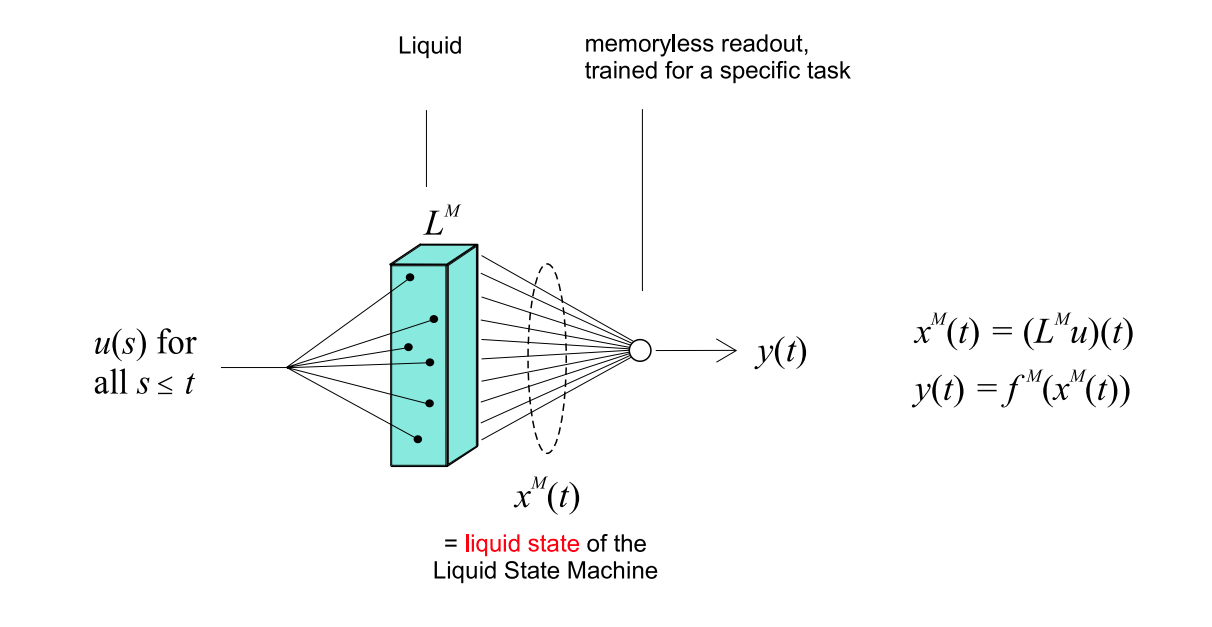
\includegraphics[width=0.8\textwidth]{figs/Liquid-state.png}
    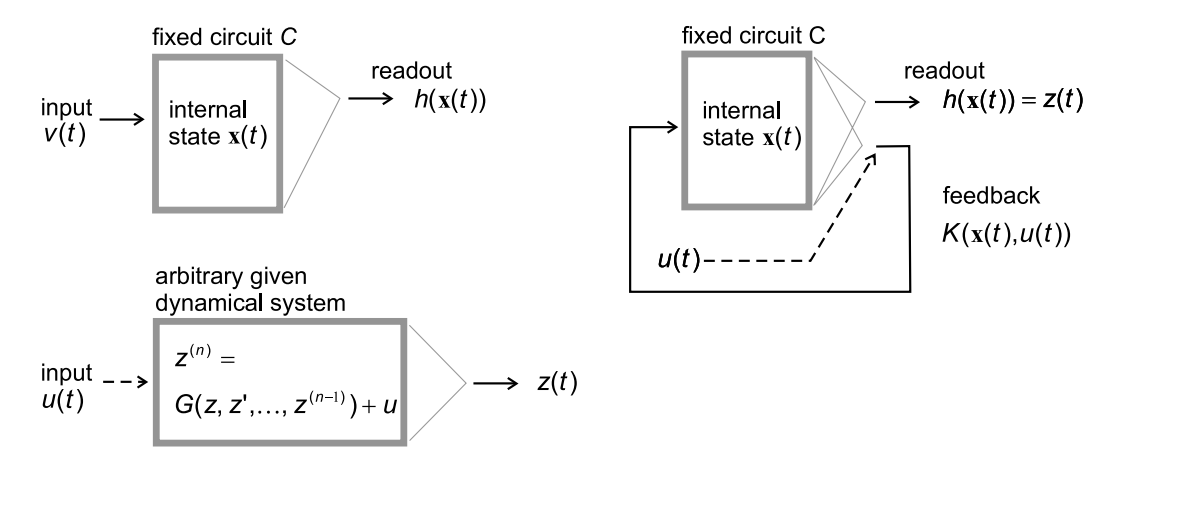
\includegraphics[width=0.8\textwidth]{figs/liquid-state-2.png}

    \caption{Liquid State Machine architecture}
    \label{fig:lsm}
\end{figure}

\subsection{Next generation reservoir computing}
Based on \autocite{Gauthier2021}.

\begin{figure}[H]
    \centering
    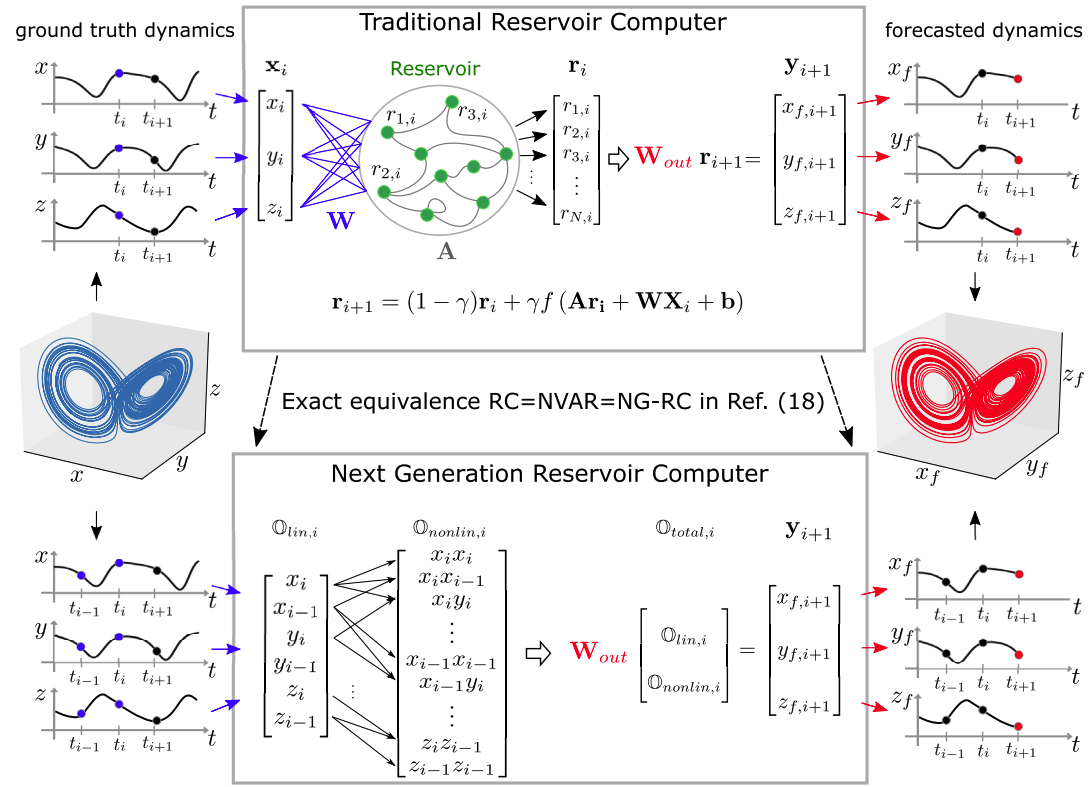
\includegraphics[width=0.8\textwidth]{figs/next-generation.png}
    \caption{ A traditional RC is implicit in an NG-RC. (top) A traditional RC processes time-series data associated with a strange attractor (blue, middle left)
        using an artificial recurrent neural network. The forecasted strange attractor (red, middle right) is a linear weight of the reservoir states. (bottom) The NGRC performs a forecast using a linear weight of time-delay states (two times shown here) of the time series data and nonlinear functionals of this data
        (quadratic functional shown here).}
    \label{fig:ng-rc}
\end{figure}

The reservoir is a
dynamic system whose dynamics can be represented by:
\begin{equation}
    \mathbf{r}_{i+1} = (1 - \gamma) \mathbf{r}_i + \gamma f \big(\mathbf{A} r_i + \mathbf{W}_{in} \mathbf{X}_i + b \big)
\end{equation}

Where:

\( r_i = [r_i^1, r_i^2, \ldots, r_i^N]^T \in \mathbb{R}^{N \times 1} \) is the reservoir state at time step \(i\),

The output layer expresses the RC output \(\mathbf{Y}_{i+1}\) as a linear
transformation of a feature vector \(\mathbf{O}_{total,i+1}\), constructed from the
reservoir state \(\mathbf{r}_{i+1}\), through the relation:
\begin{equation}
    \mathbf{Y}_{i+1} = \mathbf{W}_{out} \mathbf{O}_{total,i+1}
\end{equation}

Where:
\begin{itemize}[noitemsep, leftmargin=4cm, label={}]
    \item [\(\mathbf{O}_{total,i+1} \in \mathbb{R}^{M \times 1}\)] -- is the feature vector at time step \(i+1\),
    \item [\(\mathbf{W}_{out} \in \mathbb{R}^{p \times M}\)] -- is the output weight matrix,
    \item [\(M\)] -- is the size of the feature vector.
\end{itemize}


The RC is trained using supervised training via regularized least-squares regression. Here, the training data points generate a block of data contained in \(\mathbf{O}_{total}\) and we match \(\mathbf{Y}\) to the desired output \(\mathbf{Y}_d\) in a least-square sense using Tikhonov regularization so that \(\mathbf{W}_{out}\) is given by

\begin{equation}
    \mathbf{W}_{out} = \mathbf{Y}_d \mathbf{O}_{total}^T (\mathbf{O}_{total} \mathbf{O}_{total}^T + \alpha \mathbf{I})^{-1}
\end{equation}

A different approach to RC is to move the nonlinearity from the reservoir to the output layer. In this case, the reservoir nodes are chosen to have a linear activation function \(f(\mathbf{r}) = \mathbf{r}\), while the feature vector \(\mathbf{O}_{total}\) becomes nonlinear. A simple example of such RC is to extend the standard linear feature vector to include the squared values of all nodes, which are obtained through the Hadamard product \( \mathbf{r} \odot \mathbf{r} =  [r_1^2, r_2^2, \ldots, r_N^2]^T \)

\begin{equation}
    \mathbf{O}_{total} = \mathbf{r} \oplus (\mathbf{r} \odot \mathbf{r}) = [r_1, r_2, \ldots, r_N, r_1^2, r_2^2, \ldots, r_N^2]^T
\end{equation}
Where:
\begin{itemize}[noitemsep, leftmargin=4cm, label={}]
    \item [\(\oplus\)] -- is the concatenation operator.

\end{itemize}
Here, \(\mathbf{O}_{total} = c \cdot \mathbf{O}_{linear} \oplus \mathbf{O}_{nonlinear}\), where \(c\) is a constant
and \(\mathbf{O}_{nonlinear}\) is a nonlinear part of the feature vector. Like a traditional RC, the output is obtained using these features.

The linear features \(\mathbf{O}_{linear,i}\) at time step \(i\) is composed of observations of the input vector \(\mathbf{X}\) at the current and at \(k-1\) previous times steps spaced by \(s\), where \((s-1)\) is the number of skipped steps between consecutive observations. If \(\mathbf{X}_i = [x_{1,i}, x_{2,i}, \ldots, x_{d,i}]^T\) is a \(d\)-dimensional vector, \(\mathbf{O}_{linear,i}\) has \(d \cdot k\) components, and is given by

\begin{equation}
    \mathbf{O}_{linear,i} = \mathbf{X}_i \oplus \mathbf{X}_{i-s} \oplus \mathbf{X}_{i-2s} \oplus \ldots \oplus \mathbf{X}_{i-(k-1)s}
\end{equation}

Based on the general theory of universal approximators, \(k\) should be taken to be infinitely large. However, it is found in practice that the Volterra series converges rapidly, and hence truncating \(k\) to small values does not incur large error. This can also be motivated by considering numerical integration methods of ordinary differential equations where only a few subintervals (steps) in a multistep integrator are needed to obtain high accuracy. We do not subdivide the step size here, but this analogy motivates why small values of \(k\) might give good performance in the forecasting tasks considered below.

An important aspect of the NG-RC is that its warm-up period only contains \(sk\) time steps, which are needed to create the feature vector for the first point to be processed.

The nonlinear part \(\mathbf{O}_{nonlinear}\) of the feature vector is a nonlinear function of \(\mathbf{O}_{linear}\). While there is great flexibility in choosing the nonlinear functionals, we find that polynomials provide good prediction ability. Polynomial functionals are the basis of a Volterra representation for dynamical systems and hence they are a natural starting point. We find that low-order polynomials are enough to obtain high performance.
All monomials of the quadratic polynomial, for example, are captured by the outer product \(\mathbf{O}_{linear} \otimes \mathbf{O}_{linear}\), which is a symmetric
matrix with \((dk)^2\) elements. A quadratic nonlinear feature vector \(\mathbf{O}^{(2)}_{nonlinear}\), for example, is composed of the \((dk)(dk+1)/2\) unique monomials of \(\mathbf{O}_{linear} \otimes \mathbf{O}_{linear}\), which are given by the upper triangular elements of the outer product tensor. We define \(\lceil \otimes \rceil\) as the operator that collects the unique monomials in a vector. Using this notation, a \(p\)-order polynomial feature vector is given by

\begin{equation}
    \mathbf{O}^{(p)}_{nonlinear} =  \underbrace{\mathbf{O}_{linear} \lceil \otimes \rceil \mathbf{O}_{linear} \lceil \otimes \rceil \ldots \lceil \otimes \rceil \mathbf{O}_{linear} }_{p \text{ times}}
\end{equation}
The total feature vector used for the Lorenz63 forecasting task is given by
\begin{equation}
    \mathbf{O}_{total} = c \cdot \mathbf{O}_{linear} \oplus \mathbf{O}_{linear}  \oplus  \mathbf{O}^{(2)}_{nonlinear}
\end{equation}

To allow the NG-RC to focus on the subtle details of this process, we use a simple Euler-like integration step as a lowest-order approximation to a forecasting step by modifying Eq. 2 so that the NG-RC learns the difference between the current and future step. To this end, Eq. 2 is replaced by
\begin{equation}
    \mathbf{X}_{i+1} = \mathbf{X}_i + \mathbf{W}_{out} \mathbf{O}_{total,i}
\end{equation}

\section{Memristors in reservoir computing}

\subsection{Reservoir computing using dynamic memristors for temporal information processing}
Based on \autocite{Du2017,Hwang2025}.

\begin{figure}[H]
    \centering
    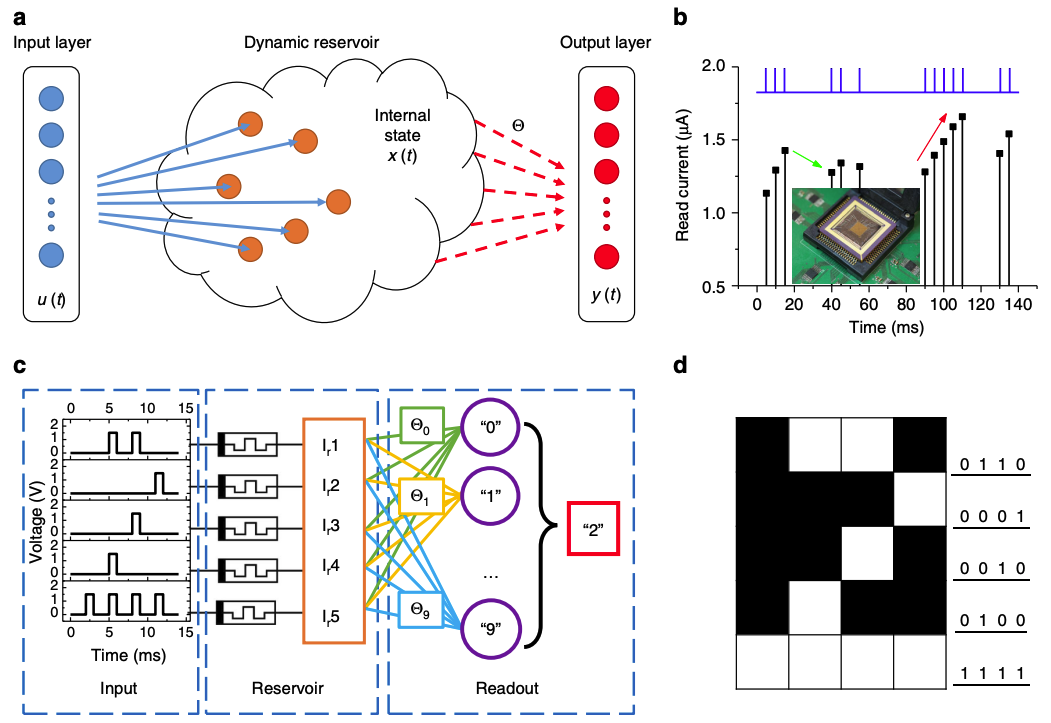
\includegraphics[width=\textwidth]{figs/reservoir-memristor-1.png}

    \caption{Reservoir computing system based on a memristor array. (a) Schematic of an RC system, showing the reservoir with internal dynamics and a readout function. Only the weight matrix \(\Theta\) connecting the reservoir state x(t) and the output y(t) needs to be trained. (b) Response of a typical WOx memristor to a pulse stream with different time intervals between pulses. Inset: image of the memristor array wired-bonded to a chip carrier and mounted on a test board. (c) Schematic of the RC system with pulse streams as the inputs, the memristor reservoir and a readout network. For the simple digit recognition task of \( 5 \times 4 \) images, the reservoir consists of 5 memristors. (d) An example of digit 2 used in the simple digit analysis.}
    % \label{fig:memristor-rc}
\end{figure}
\begin{figure}[H]
    \centering
    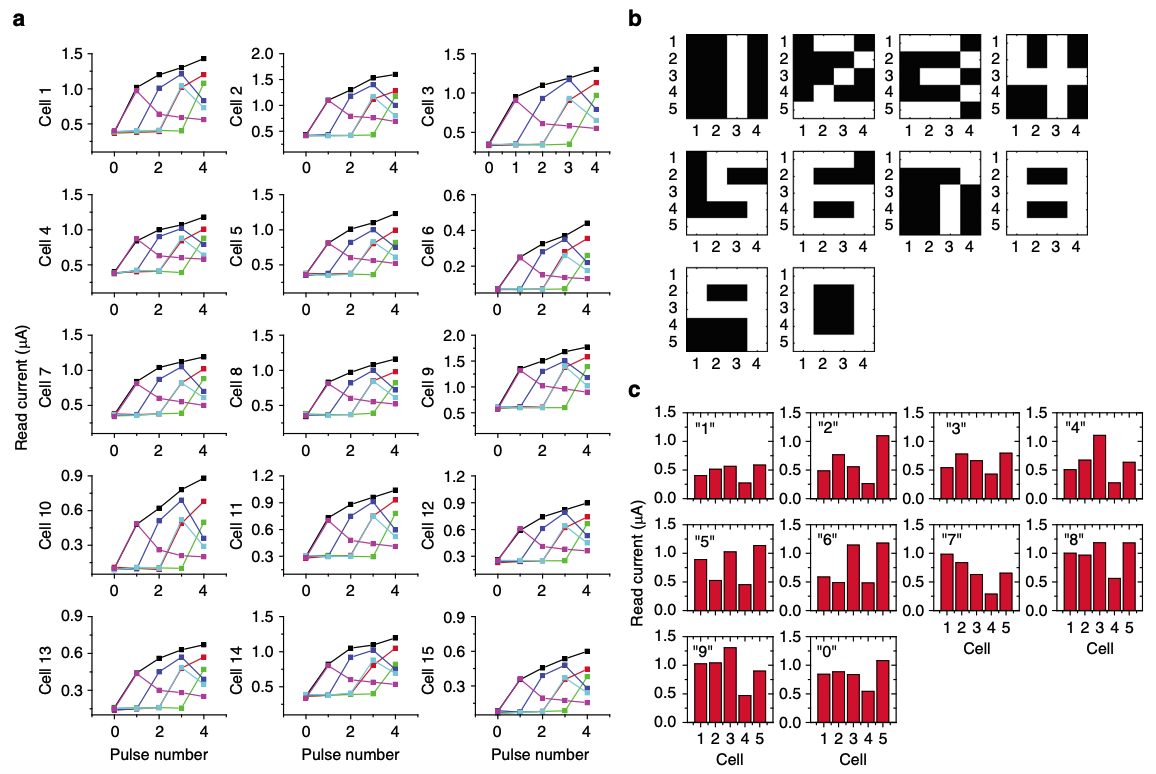
\includegraphics[width=\textwidth]{figs/reservoir-memristor-2.png}

    \caption{Reservoir states used to differentiate different temporal inputs. (a) The response of 15 memristors from the array to 6 different pulse streams (black: [1 1 1 1], purple: [1 0 0 0], blue: [0 1 1 0], red: [0 0 1 1], cyan: [0 0 1 0], green: [0 0 0 1]), showing similar response from all devices, as well as device variations. (b) Images of the 10 digits used in this test. (c) Experimentally measured reservoir states after the memristors are subjected to the 10 inputs. The reservoir state is reflected as the read currents of the 5 memristors forming the reservoir.}
    % \label{fig:memristor-rc}
\end{figure}
\begin{figure}[H]
    \centering
    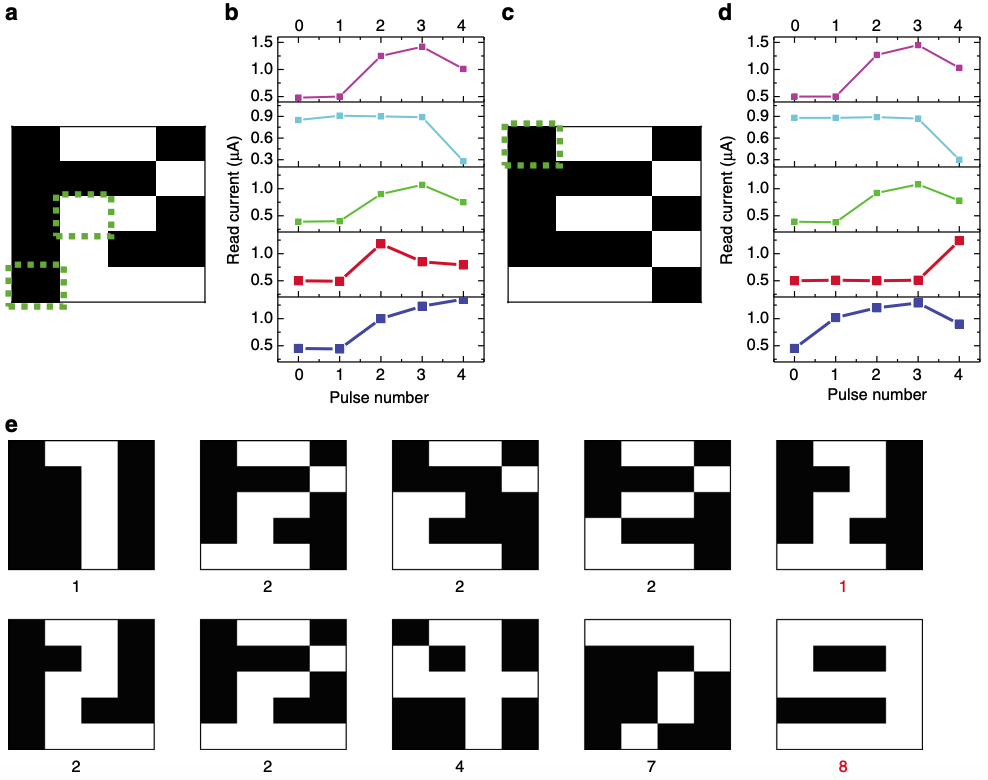
\includegraphics[width=\textwidth]{figs/reservoir-memristor-3.png}

    \caption{Recognition of noisy images. (a, c) Distorted images of digits 2 and 3 are generated by adding noise to the original data at locations marked by the dashed squares. (b, d) Corresponding reservoir states for these two inputs, showing differences in the two digits can be clearly captured by the memristors corresponding to the last two rows. (e) Recognition results of noisy digits. The RC system output, e.g., the predicted digit is shown below each case. The distorted images are generated by adding noise to the original training samples. The system can still successfully identify the majority of the distorted images without additional training, until too much noise is added as in the last two cases where the incorrect classifications are marked in red}
    % \label{fig:memristor-rc}
\end{figure}


\begin{figure}[H]
    \centering
    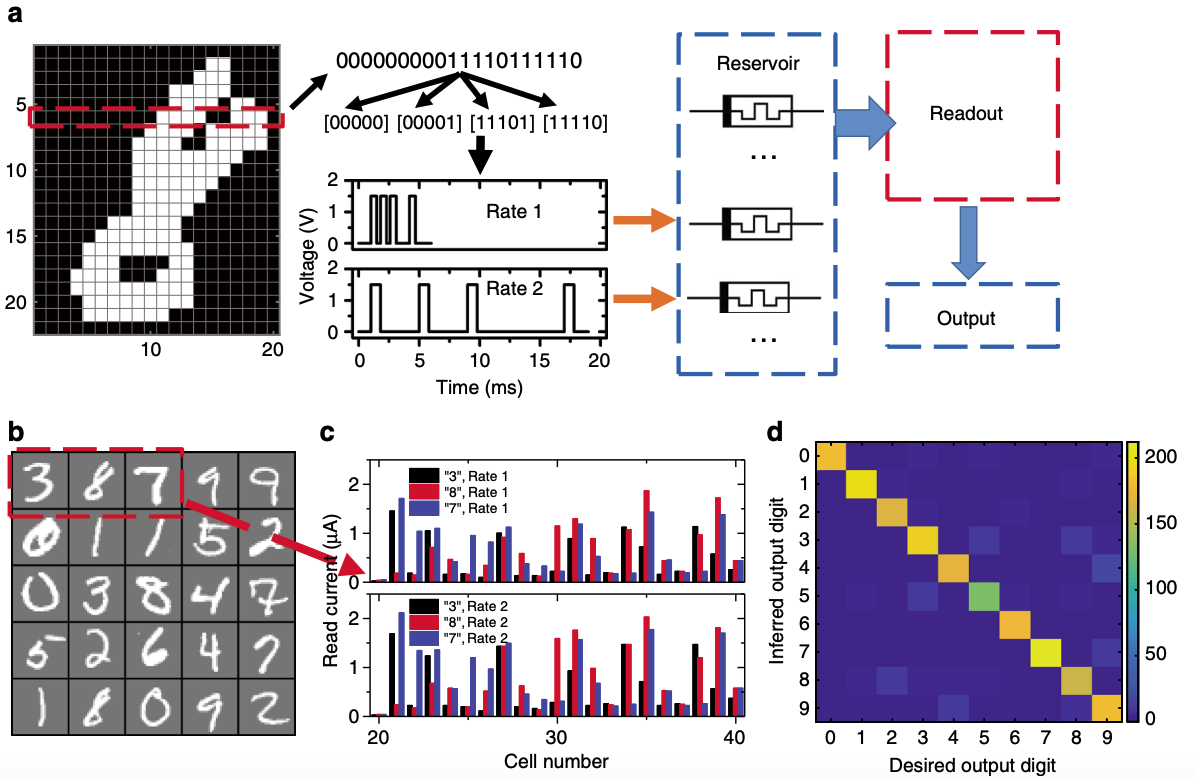
\includegraphics[width=\textwidth]{figs/reservoir-memristor-4.png}

    \caption{Handwritten digit recognition using a memristor-based RC system. (a) The process flow. The original digit image is first converted into pulse streams and fed to the memristor-based reservoir at different rates. The recognition result is generated after feeding the reservoir state to a trained readout function. (b) Some examples from the MNIST database. (c) Reservoir states corresponding to the three examples in (b) at two input rates (rate 1: timeframe width 0.8 ms, with pulse of 1.5 V, 0.5 ms; rate 2: timeframe width 4 ms, with pulses of 1.5 V, 0.8 ms), showing significant differences in the reservoir states. (d) False color confusion matrix showing the experimentally obtained classification results from the RC system vs. the desired outputs. The occurrence of the predicted output for each test case is represented by colors shown in the color scale. A recognition accuracy of 88.1\% was obtained from the reservoir consisting of only 88 memristors.}
    % \label{fig:memristor-rc}
\end{figure}
\section{Potential next steps in memristor-based reservoir computing}

\begin{itemize}
    \item Investigation of possible architectures for memristor-based reservoir computing systems, including hybrid approaches that combine memristors with other types of hardware.
    \item Development of training algorithms specifically designed for memristor-based reservoirs, taking into account the unique properties of memristors.
    \item Exploration of possibility of robust modelling of circuits with memristors within reservoir computing framework.
\end{itemize}

\section{Simulation results}

The experimental investigation commenced with comprehensive computational simulations employing the memristor MMS  model.

For the evaluation of the proposed reservoir computing architecture, the standardized MNIST (Modified National Institute of Standards and Technology) dataset was utilized, comprising grayscale images of handwritten digits with dimensions of 28×28 pixels. This benchmark dataset represents a fundamental test case for pattern recognition systems and enables direct comparison with existing neuromorphic computing paradigms.

\subsection{Row-Wise Input Encoding Methodology}

The initial phase of the simulation protocol involved a row-wise decomposition strategy, described in \autocite{Du2017} for processing the input images. Specifically, each 28×28 pixel image was segmented into 28 discrete rows, with each row being processed sequentially through the reservoir architecture. This decomposition approach facilitated the implementation of a reservoir configuration comprising 28 memristive elements, where each memristor corresponded to a distinct spatial position within the input row vector.

The encoding of pixel information into the temporal domain was accomplished through a voltage-based pulse amplitude modulation scheme. Each grayscale pixel value, normalized within the range [0, 1], was mapped to a corresponding voltage amplitude in the range [0, V\textsubscript{max}] volts, where V\textsubscript{max} represents the maximum applied voltage determined by the operational constraints of the memristive devices. This linear mapping function can be expressed as:

\begin{equation}
    V_{\text{pixel}}(i,j) = V_{\text{max}} \cdot \frac{I(i,j)}{255}
\end{equation}
where \(I(i,j)\) denotes the grayscale intensity value at pixel position \((i,j)\), and \(V_{\text{pixel}}(i,j)\) represents the corresponding encoded voltage amplitude.

\subsubsection{Results}
For the provided row-wise input encoding methodology, the memristor-based reservoir computing system achieved a classification accuracy of 60.37\% on the MNIST dataset. This performance metric underscores the low efficacy of the proposed architecture in leveraging the intrinsic dynamics of memristive devices for temporal information processing tasks.

% \subsection{Convolutional Input Encoding Methodology}

\subsection{Patch-Based Feature Extraction and Memristor Reservoir Processing}

Building upon the row-wise processing paradigm, a more sophisticated approach was developed employing a patch-based feature extraction methodology combined with memristor reservoir computing. This technique leverages local spatial correlations within the input images while maintaining computational efficiency through systematic spatial subsampling.

\subsubsection{Spatial Patch Extraction Algorithm}

The foundation of this approach rests upon a sliding window mechanism for extracting overlapping or non-overlapping rectangular patches from the input images. The patch extraction function implements a systematic traversal of the image space according to the following algorithmic procedure:



Given an input image \(\mathbf{I} \in \mathbb{R}^{H \times W}\) where \(H\) and \(W\) denote the height and width respectively, the extraction process generates a set of patches \(\mathcal{P} = \{P_1, P_2, ..., P_N\}\) where each patch \(P_i \in \mathbb{R}^{k_h \times k_w}\) represents a local spatial region of dimensions \(k_h \times k_w\) (the kernel size). The extraction follows a raster scan pattern with a specified stride parameter \(s\) that controls the spatial sampling density.

The mathematical formulation of the patch extraction can be expressed as:

\begin{equation}
    P_{m,n} = \mathbf{I}[is:(is+k_h-1), js:(js+k_w-1)]
\end{equation}

where the indices \((m,n)\) correspond to the patch coordinates in the output grid, and:
\begin{align}
    i & = 1 + m \cdot s, \quad m \in \{0, 1, ..., \lfloor\frac{H-k_h}{s}\rfloor\} \\
    j & = 1 + n \cdot s, \quad n \in \{0, 1, ..., \lfloor\frac{W-k_w}{s}\rfloor\}
\end{align}

Each extracted patch is subsequently vectorized through a flattening operation, transforming the 2D patch into a 1D feature vector of length \(k_h \cdot k_w\):

\begin{equation}
    \vec{p}_i = \text{vec}(P_i) \in \mathbb{R}^{k_h \cdot k_w}
\end{equation}

\subsubsection{Implementation Parameters for MNIST Processing}

For the specific case of MNIST digit classification, the following hyperparameters were empirically determined to optimize the balance between feature resolution and computational efficiency:

\begin{itemize}
    \item \textbf{Kernel dimensions}: \((k_h, k_w) = (5, 5)\), yielding 25-dimensional feature vectors per patch
    \item \textbf{Stride}: \(s = 3\) pixels, providing moderate spatial overlap between adjacent patches
    \item \textbf{Image dimensions}: \((H, W) = (28, 28)\) pixels (standard MNIST format)
\end{itemize}

These parameters result in a systematic decomposition of each image into a grid of patches with dimensions:

\begin{align}
    n_{\text{patches}}^h              & = \lfloor\frac{28 - 5}{3}\rfloor + 1 = 8                \\
    n_{\text{patches}}^w              & = \lfloor\frac{28 - 5}{3}\rfloor + 1 = 8                \\
    n_{\text{patches}}^{\text{total}} & = n_{\text{patches}}^h \times n_{\text{patches}}^w = 64
\end{align}

This configuration effectively transforms each 784-dimensional input image (28×28 pixels) into 64 localized feature patches, each containing 25 pixels of spatial information.

\subsubsection{Temporal Encoding via Carrier Wave Modulation}

The proposed methodology involves the encoding of patch information through amplitude-modulated carrier waves. For each patch vector \(\vec{p}_i\), a time-varying voltage signal is generated using the following carrier wave generation scheme:

\begin{equation}
    V_{\text{carrier}}(t) = A(t) \cdot \Pi\left(\frac{t \bmod T_{\text{period}}}{D \cdot T_{\text{period}}}\right)
\end{equation}

where:
\begin{itemize}
    \item \(A(t)\) represents the amplitude modulation function derived from the patch pixel values
    \item \(\Pi(\cdot)\) denotes the rectangular pulse function
    \item \(T_{\text{period}} = 10^{-5}\) seconds (10 microseconds) is the carrier period
    \item \(D = 0.8\) is the duty cycle, resulting in 8 microseconds on-time and 2 microseconds off-time
    \item The sampling frequency \(f_s = 10^7\) Hz (10 MHz) ensures adequate temporal resolution
\end{itemize}

The amplitude modulation encodes each pixel value within the patch as a discrete voltage level, creating a multi-level pulse train that preserves the spatial information in the temporal domain. This encoding is particularly well-suited for memristor dynamics, as it exploits the devices' inherent integration capabilities.


\subsubsection{Feature Vector Construction and Augmentation}

The final feature representation for each image is constructed by aggregating the terminal states of all memristors after processing their respective patches:

\begin{equation}
    \mathbf{x}_j = [x_1^{\text{final}}, x_2^{\text{final}}, ..., x_{64}^{\text{final}}, 1]^T \in \mathbb{R}^{65}
\end{equation}

where \(x_i^{\text{final}} = x_i(t_{\text{max}})\) represents the final state of the memristor processing patch \(i\), and the additional unity element serves as a bias term for subsequent linear classification layers.

This feature extraction process is applied systematically to the entire training dataset, resulting in a transformed feature matrix:

\begin{equation}
    \mathbf{X} = [\mathbf{x}_1, \mathbf{x}_2, ..., \mathbf{x}_N] \in \mathbb{R}^{65 \times N}
\end{equation}

where \(N\) denotes the number of training samples.

\subsubsection{Computational Complexity and Parallelization Potential}

The patch-based approach offers several computational advantages over full-image processing:

1. \textbf{Reduced dimensionality}: Each memristor processes only 25 pixels instead of 784, significantly reducing the temporal duration of input signals.

2. \textbf{Natural parallelism}: The 64 patches can be processed independently, enabling straightforward parallelization across multiple memristor units or computational cores.

3. \textbf{Memory efficiency}: The patch-wise processing requires storage of only \((n_{\text{patches}} + 1) \times N\) floating-point values for the feature matrix, compared to the original \(784 \times N\) pixel values.

The total computational time for processing a single image can be estimated as:

\begin{equation}
    T_{\text{total}} = n_{\text{patches}} \times T_{\text{patch}} + T_{\text{overhead}}
\end{equation}

where \(T_{\text{patch}}\) represents the time required for a single patch-memristor interaction, and \(T_{\text{overhead}}\) accounts for data preparation and feature aggregation operations.


\subsection{Results}

For the provided patch-based feature extraction and memristor reservoir processing methodology, the memristor-based reservoir computing system achieved a classification accuracy of 80.25\% on the MNIST dataset. This performance metric underscores higher  efficacy of the proposed architecture in leveraging localized spatial features and the intrinsic dynamics of memristive devices for temporal information processing tasks.



\printbibliography

\end{document}

